\chapter{Descripción del Trabajo}
\label{cap:descripcionTrabajo}

En este capítulo abordaremos los aspectos tanto de diseño como de implementación de nuestra aplicación...TO BE CONTINUED

\section{Previos a la implementación}

\subsection{Reunión en el Centro de Tiflotecnología e Innovación de la ONCE}

\subsection{Exactitud de los beacons}

Antes de ponernos manos a la obra con la aplicación debíamos comprobar también cómo se comportaban los beacons en cuanto a distancias. Para ello hicimos uso de pequeñas y simples aplicaciones con las que pudimos medir las distancias a los beacons en diferentes situaciones. 

\begin{figure}[t]
	\centering
	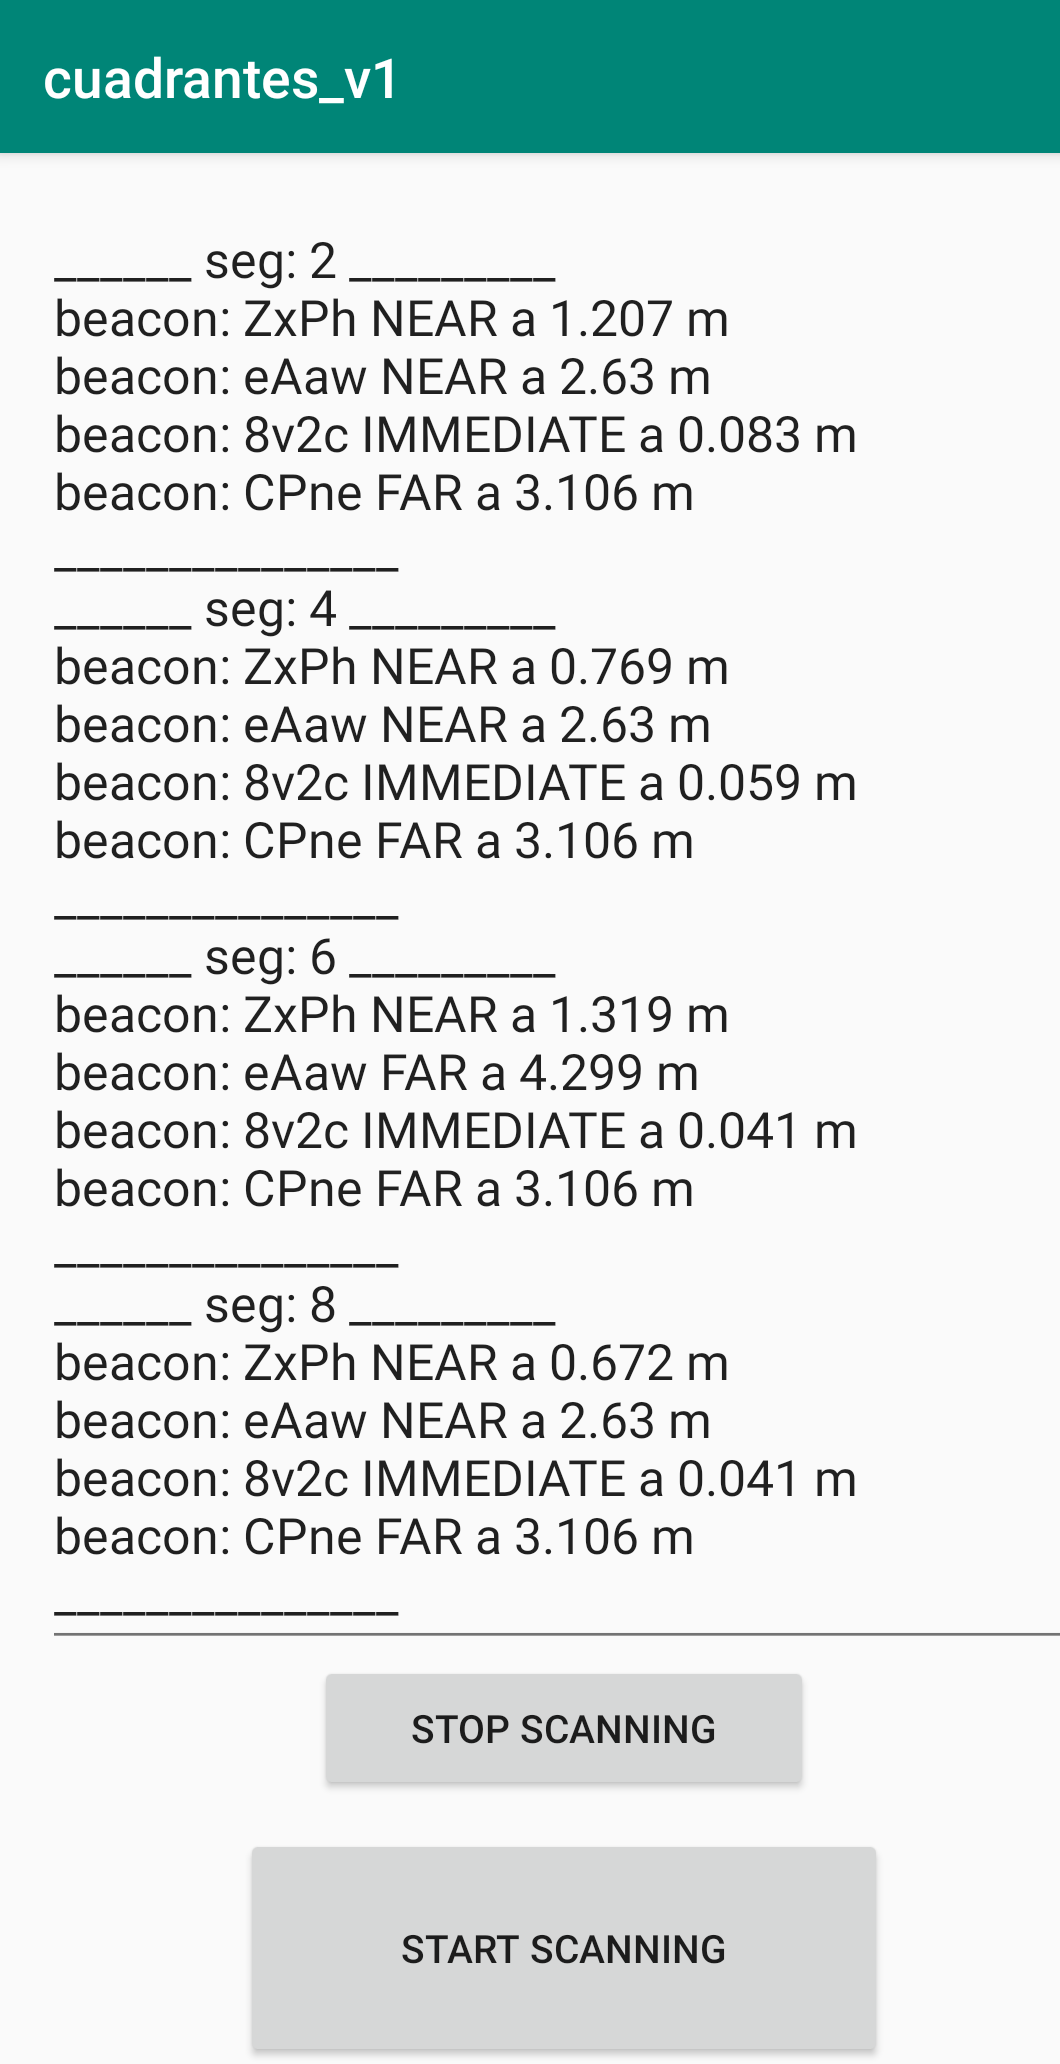
\includegraphics[width=0.4\textwidth]{Imagenes/Descripciondeltrabajo/cuadrantes_v1}
	\caption{Interfaz de la aplicación cuadrantes v1.}
	\label{fig:cuadrantesv1}
\end{figure}


\begin{figure}[t]
	\centering
	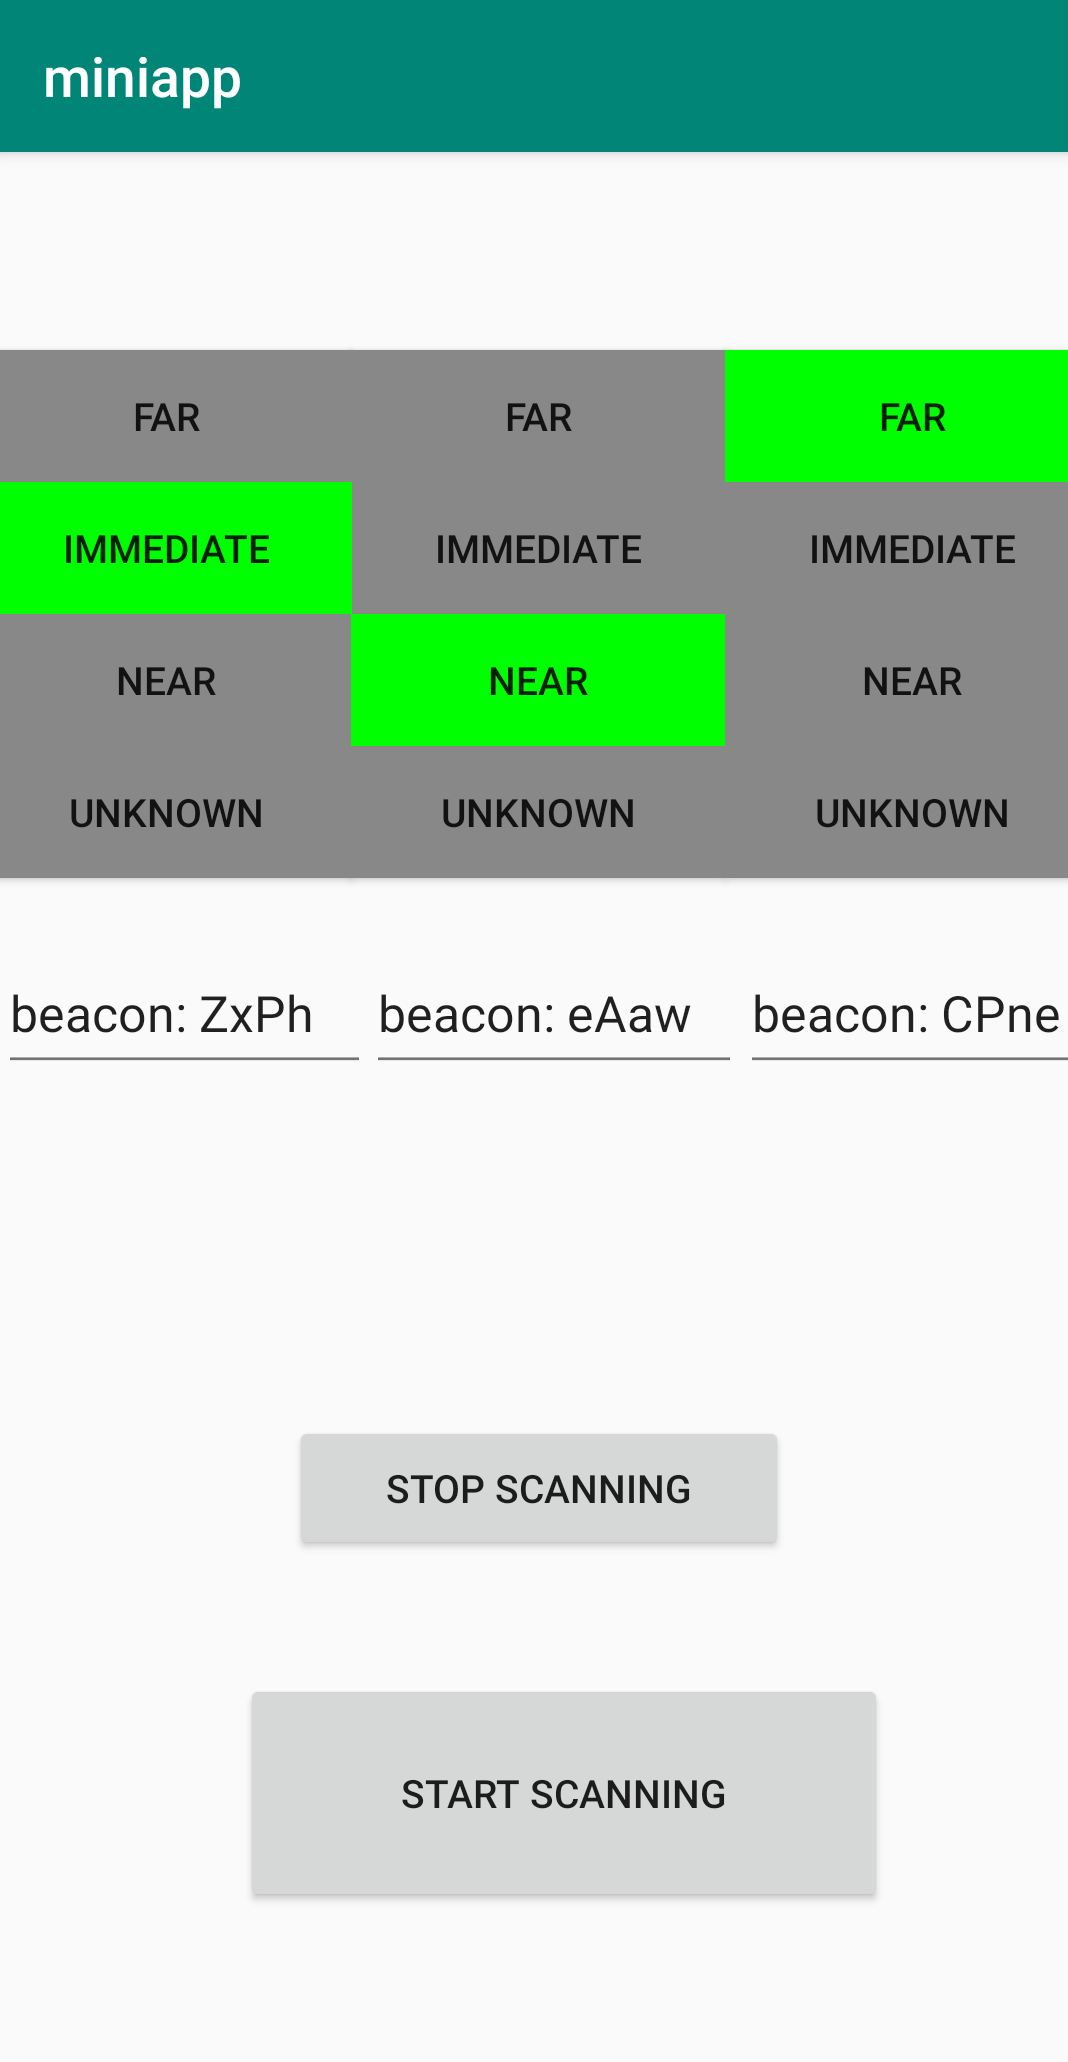
\includegraphics[width=0.4\textwidth]{Imagenes/Descripciondeltrabajo/miniapp}
	\caption{Interfaz de la aplicación miniapp. }
	\label{fig:miniapp}
\end{figure}


\begin{figure}[t]
	\centering
	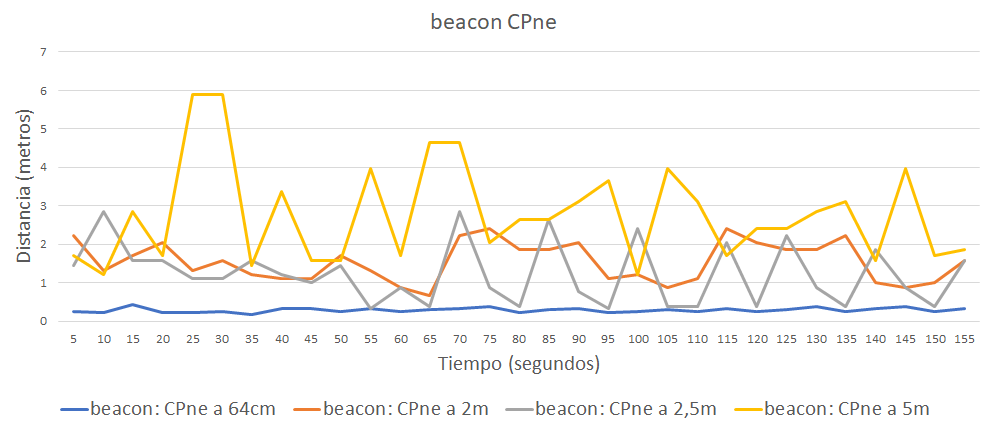
\includegraphics[width=0.7\textwidth]{Imagenes/Descripciondeltrabajo/dist_CPne}
	\caption{Gráfico con las distancias medidas al beacon CPne. }
	\label{fig:dist_CPne}
\end{figure}


\begin{figure}[t]
	\centering
	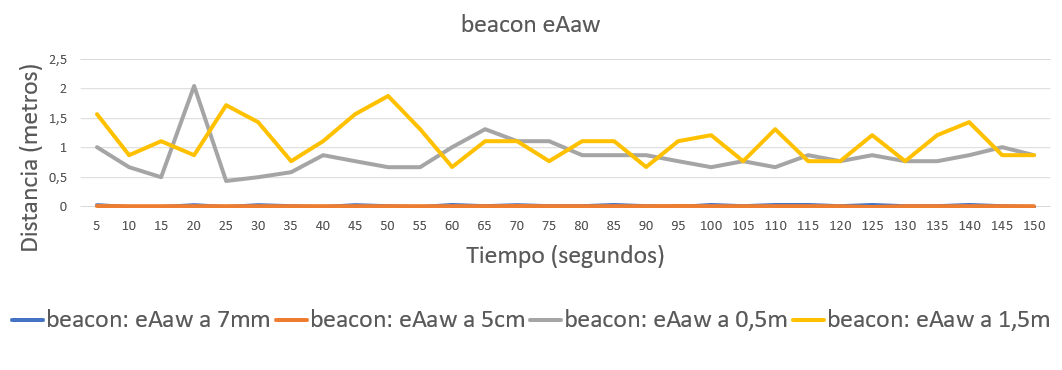
\includegraphics[width=0.7\textwidth]{Imagenes/Descripciondeltrabajo/dist_eAaw}
	\caption{Gráfico con las distancias medidas al beacon eAaw. }
	\label{fig:dist_eAaw}
\end{figure}


\begin{figure}[t]
	\centering
	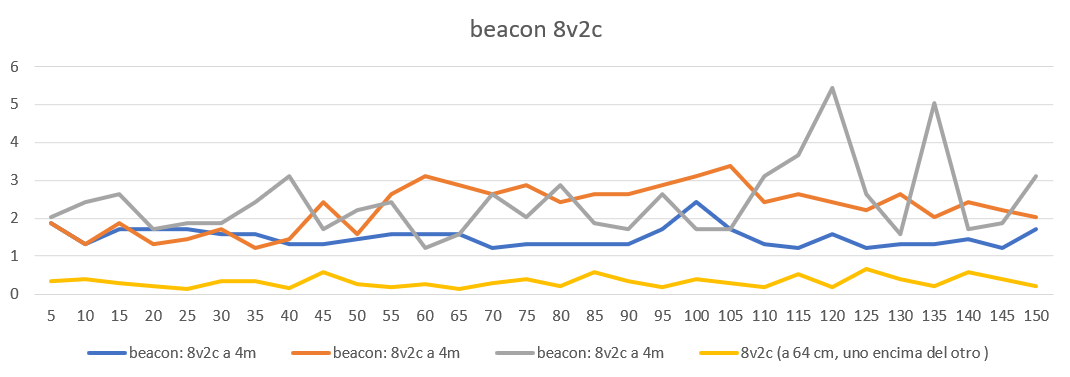
\includegraphics[width=0.7\textwidth]{Imagenes/Descripciondeltrabajo/dist_8v2c}
	\caption{Gráfico con las distancias medidas al beacon 8v2c. }
	\label{fig:dist_8v2c}
\end{figure}

\begin{figure}[t]
	\centering
	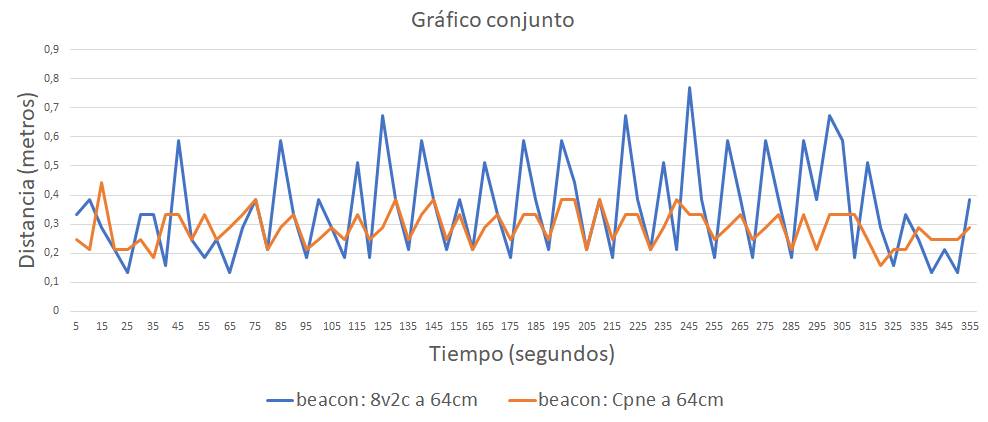
\includegraphics[width=0.7\textwidth]{Imagenes/Descripciondeltrabajo/dist_conjunto}
	\caption{Gráfico con las distancias medidas conjuntas de los beacons 8v2c y CPne, estando uno sobre otro. }
	\label{fig:dist_conjunto}
\end{figure}
